In \Cref{sec:validation} it was shown that the background distributions are adequatly represented in simulation,
which proves that the analysis setup on simulation is valid for data.
It was also seen that the \Mbc fitter is able to extract values consistent with zero, where no \BtoXsgamma signal was expected.
The analysis strategy in \Cref{sec:final_optimisation,sec:fitting_mbc,sec:background_subtraction} does not strongly depend on the signal model.
In fact, no strong assumptions are made about the signal shape at any point in the analysis so far.
Therefore, following the fitting and background subtraction procedures, the number of \BtoXsgamma events as a function of \EB in the analysed Belle~II data sample can be evaluated. 

In order to transform the measured numbers of \BtoXsgamma events to partial branching fractions of \BtoXsgamma decays, efficiency corrections and unfolding is necessary.
In this section, the expected signal efficiency and \EB resolution of \BtoXsgamma events will be investigated.
The hybrid-signal model will then be used to derive unfolding correction factors.

\subsection{Efficiency of \texorpdfstring{\BtoXsgamma}{B->Xs gamma} decays}\label{sec:signal_efficiency}

The \BtoXsgamma selection efficiency is evaluated using Belle~II simulation and corrected
based on the studies that have been discussed in \Cref{sec:corrections}.
The signal efficiency is firstly assumed to be factorisable:
\begin{equation}\label{eq:factorisable_signal_efficiency}
    \varepsilon_{\BtoXsgamma} = \varepsilon_{\mathrm{FEI}} \times \varepsilon_{\mathrm{selection}},
\end{equation}
where $\varepsilon_{\mathrm{FEI}}$ is the \FEI tagging efficiency and 
$\varepsilon_{\mathrm{selection}}$ is the selection efficiency related to requirements shown in \Cref{sec:selection_summary}.
The factorisation assumption is a valid one as $\varepsilon_{\mathrm{FEI}}$  is related to the reconstruction of the tag-\B meson,
whereas $\varepsilon_{\mathrm{selection}}$ is fully a signal-\B meson quantity.

The \FEI tagging efficiency is evaluated as:
\begin{equation}\label{eq:fei_tagging_efficiency}
    \varepsilon_{\mathrm{FEI}} = \frac{N(\BtoXsgamma)_{\mathrm{good~tags}}}{N(\BtoXsgamma)_{\mathrm{untagged}}}
\end{equation}
The numerator, $N(\BtoXsgamma)_{\mathrm{good~tags}}$, is equal to the number of \BtoXsgamma events associated with good tag-\B mesons after running \FEI. 
It is evaluated using the good-tag definition in \Cref{sec:good_tag_definition}.
The denominator, $N(\BtoXsgamma)_{\mathrm{untagged}}$, is equal to the number of \BtoXsgamma events on an equivalent sample, where \FEI is not run.
In both cases the hybrid signal-model is used.

The evaluated tagging efficiency is shown in \Cref{fig:epsilon_fei}.
The efficiency is evaluated as a function of $\tilde{\EB}$, which is adopted only here to denote that the \textit{true} photon energy is used, 
as opposed to the reconstructed value.
This is done, as the untagged inclusive sample cannot have a meaningful comparison in terms of reconstructed \EB.
It can be seen that the efficiency increases with $\tilde{\EB}$, but the overall increase is roughly 10\% throughout the considered range.
As direct connection between $\tilde{\EB}$ and $\EB$ is difficult to evaluate, the average efficiency value is chosen as the tagging efficiency:
\begin{equation}\label{eq:avg_efficiency_fei}
    \varepsilon_{\mathrm{FEI}} = 0.006659 \pm 0.000006,
\end{equation}
where the uncertainty is fully statistical.
The signal-modelling uncertainty is expected to be small, because any deviations would be suppressed in the rattio in \Cref{eq:fei_tagging_efficiency}.
\begin{figure}[htbp!]
    \centering
    \subcaptionbox{\label{fig:epsilon_fei}}{
        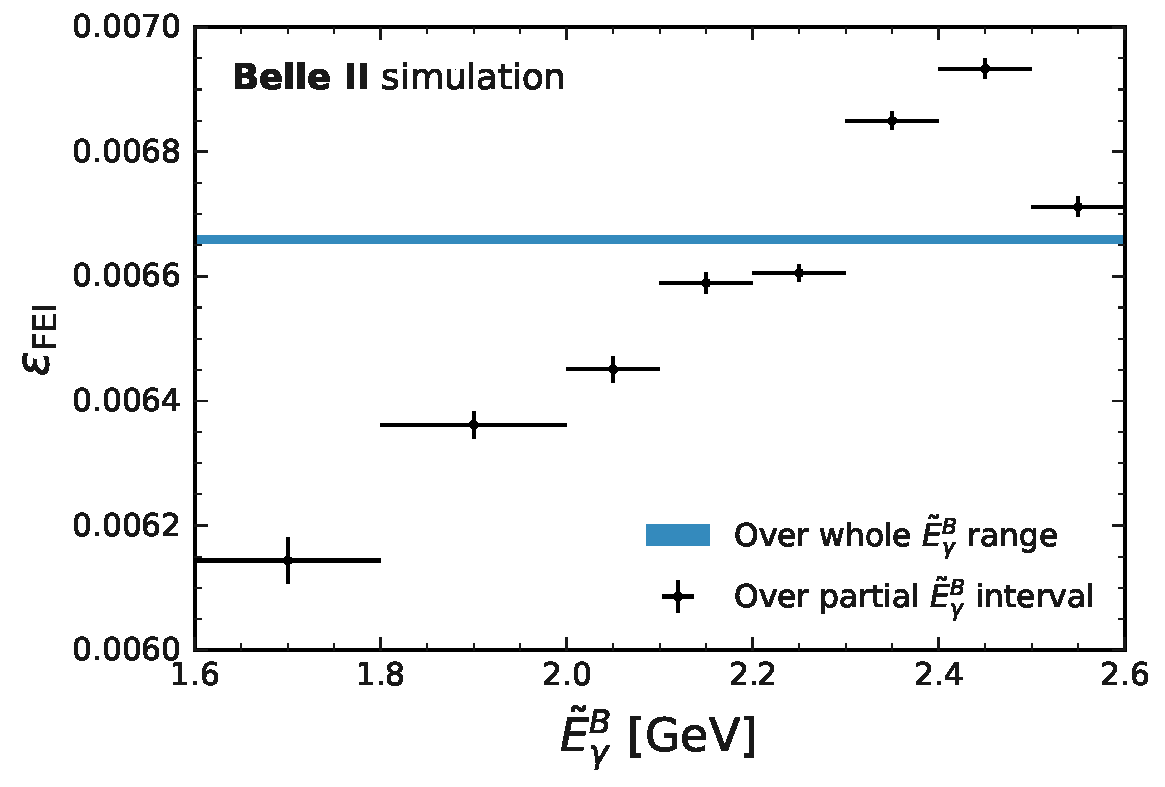
\includegraphics[width=0.41\textwidth]{figures/signal_validation/epsilon_fei.pdf}
    }
    \subcaptionbox{\label{fig:epsilon_selection}}{
        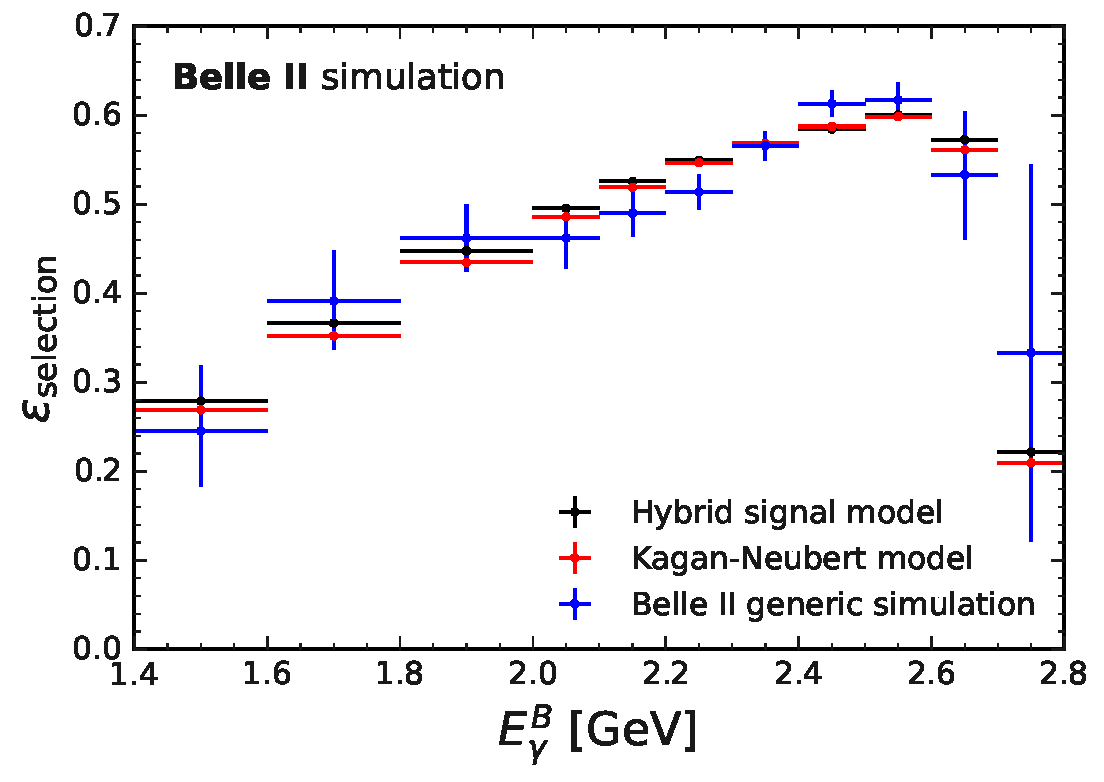
\includegraphics[width=0.41\textwidth]{figures/signal_validation/selection_efficiency.pdf}
    }
    \caption{\label{fig:epsilon} The efficiency evaluation of \BtoXsgamma events in simulated samples based on the two factorised components in
    \Cref{eq:factorisable_signal_efficiency}.
    $\epsilon_{\mathrm{FEI}}$, shown in \Cref{fig:epsilon_fei}, is seen to vary lightly, no more than 10\% accross the $\tilde{\EB}$ range.
    Note that $\tilde{\EB}$ is used, as opposed to \EB, to represenet `true' photon energy (generated for simulation), 
    as opposed to the reconstructed value.
    $\epsilon_{\mathrm{selection}}$, shown in \Cref{fig:epsilon_selection} for three different models,
    grows with \EB approximately linearly and starts to drop at $\EB\approx2.6~\gev$.
    The three models show consistent results, strengthening the argument of a signal-model independent analysis.
    }
\end{figure}

The \BtoXsgamma signal efficiency is evaluated using three different signal models as:
\begin{equation}\label{eq:signal_efficiency}
    \varepsilon_{\mathrm{selection}} = \frac{N(\BtoXsgamma)_{\mathrm{after~selection}}}{N(\BtoXsgamma)_{\mathrm{before~selection}}},
\end{equation}
here $N(\BtoXsgamma)_{\mathrm{after(before)~selection}}$ is the count of \BtoXsgamma events in the \FEI tagged sample with(without) 
the background suppression selections in this analysis, given in \Cref{tab:interative_optimisation}.
This is evaluated on three models: the Kagan-Neubert model, the Belle~II generic-\MC signal model, and the hybrid-signal model.
The results are shown in \Cref{fig:epsilon_selection}.
All three models show compatible results.
The $\varepsilon_{\mathrm{selection}}$ grows approximately linearly from 30\% at 1.4~\gev to 60\% at 2.6~\gev and then drops sharply.
In this analysis, the values from hybrid signal-model are used as central values of the efficiency.

These results, summarised in \Cref{fig:epsilon} allow to evaluate the simulated efficiency based on \Cref{eq:factorisable_signal_efficiency}.

\subsection{Validation of \texorpdfstring{\BtoXsgamma}{B->Xs gamma} efficiency}\label{sec:validation_efficiency}



